\begin{pastexam}[label={px:gw3-110-ds-03}]{關務三等資訊處理 110 年 第三題}
（申論）

$\forall k \in$ N-\{1\}，若有一棵 k 元樹（k\_ary tree）其中分支度（degree）為 i 的節點數為 i 個，i = 1, 2, ..., k，請問
該 k 元樹其葉節點數 L(k)為何？（15 分）
\end{pastexam}

\begin{pastsoln}
答案：$L(k) = \dfrac{(k-1)k(k+1)}{3} + 1 = \dfrac{k^3 - k}{3} + 1$。

\textbf{推導。} 樹裡的分支度指子節點個數。 葉節點分支度為 $0$；分支度 $i$ 的節點有 $i$ 個（$i = 1, \ldots, k$）。 用兩種
方法數節點總數 $n$（和資結書定理~7.2 $n_0 = n_2 + 1$ 的證法相同）：
\begin{itemize}
\item 按分支度分類：$n = L + \sum_{i=1}^{k} i = L + \dfrac{k(k+1)}{2}$。
\item 按邊數：除了根，每個節點恰好有一條邊連到父節點，所以邊數是 $n - 1$；另一方面每條邊由父節點「發出」，
分支度 $i$ 的節點發出 $i$ 條，共 $\sum_{i=1}^{k} i \cdot i = \dfrac{k(k+1)(2k+1)}{6}$ 條。 所以
$n = 1 + \dfrac{k(k+1)(2k+1)}{6}$。
\end{itemize}
兩式相等：
\begin{align*}
L &= 1 + \frac{k(k+1)(2k+1)}{6} - \frac{k(k+1)}{2}
   = 1 + \frac{k(k+1)\bigl((2k+1) - 3\bigr)}{6} \\
  &= 1 + \frac{k(k+1)(2k-2)}{6}
   = 1 + \frac{(k-1)k(k+1)}{3}.
\end{align*}
一般公式是 $n_0 = 1 + \sum_{i \ge 1} (i-1)\, n_i$，代入 $n_i = i$ 也得到同樣結果。 $(k-1)k(k+1)$ 是三個連續整數的
乘積，必被 $3$ 整除，所以 $L(k)$ 一定是整數。

\textbf{驗證。} $k = 2$：分支度 $1$ 的節點 $1$ 個、分支度 $2$ 的節點 $2$ 個，$L(2) = \frac{1 \cdot 2 \cdot 3}{3} + 1 = 3$。
下圖就是一棵這樣的樹（$a$ 分支度 $1$，$b$、$c$ 分支度 $2$，葉子 $d, e, f$ 三個）：
\begin{center}
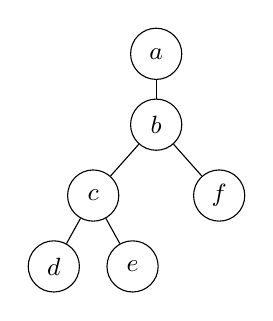
\begin{tikzpicture}[every node/.style={circle,draw,minimum size=6.5mm,inner sep=0pt,font=\small},
  level distance=9mm, level 1/.style={sibling distance=12mm}, level 2/.style={sibling distance=16mm},
  level 3/.style={sibling distance=10mm}]
\node {$a$} child {node {$b$} child {node {$c$} child {node {$d$}} child {node {$e$}}} child {node {$f$}}};
\end{tikzpicture}
\end{center}
共 $6$ 個節點、$5$ 條邊，$1 \cdot 1 + 2 \cdot 2 = 5$，吻合。 $k = 3$ 時 $L(3) = \frac{2 \cdot 3 \cdot 4}{3} + 1 = 9$；
$k = 4$ 時 $L(4) = \frac{3 \cdot 4 \cdot 5}{3} + 1 = 21$。
\end{pastsoln}
